\chapter{Domain Model}
\label{chapter:domainModel}

\section{Concepts}
\label{section:SAConcepts}
Before describing the domain model of the developed solution, it is necessary to provide a small introduction to the most important concepts from the Software Architectures course.
\subsection{Scenarios}
A scenario is used to capture and express the quality requirements of a system. The considered qualities are:
\begin{itemize}
\item Availability;
\item Interoperability;
\item Modifiability;
\item Performance;
\item Security;
\item Testability;
\item Usability;
\end{itemize}

A scenario consists of six parts \cite{bass2003software}:
\begin{itemize}
\item \textbf{Source of Stimulus:} Some entity (a human, a computer or any other actuator) that generates the stimulus;
\item \textbf{Stimulus:} A condition that arrives at the system;
\item \textbf{Environment:} The system condition when the stimulus occurs;
\item \textbf{Artifact:} Part of the system that was stimulated;
\item \textbf{Response:} Activity undertaken after the arrival of the stimulus;
\item \textbf{Response Measure:} when the response occurs, it should be measurable in some way, so the requirement can be tested;
\end{itemize}

Each Scenario uses a set of Tactics, which are design decisions used to achieve the quality requirements expressed in them. Each quality requirement has a set of commonly used tactics. For example, to assure the Security of a system, tactics such as detecting service denial or message delays (to detect attacks), or revoking access to the system (to react to an attack) are used.

\subsection{Views}
A view is a representation of a set of system elements and the relationships associated with them \cite{clements2003documenting}. This set of elements and relationships is constrained by viewtypes.

A Viewtype defines the element types and relationship types used to describe the architecture of a software system from a particular perspective. Viewtypes refine into styles.

An architectural style is a specialization of element and relation types, together with a set of constraints on how they can be used.

Views can fall into three viewtype categories:
\begin{itemize}
\item \textbf{Module Viewtype:} document the system principal units of implementation. 

The elements of this viewtype are the \textit{Modules}, which is are implementation units. 

Relationships between modules can be of type \textit{``Is-part-of''}, which defines a part-whole relationship, \textit{``Depends on''}, which defines dependency relations, and \textit{``Is-a''}, which defines a generalization/specialization relationship.

\item \textbf{Component \& Connector Viewtype:} document the system units of execution. 

The elements are the Components, which are the principal processing units and data stores, and the Connectors, which are pathways of interaction between components. 

The relationships can be of type \textit{``Attachment''}, which associate components to connectors, and \textit{``Interface''} Delegation, which associates component ports to other ports from an ``internal architecture''- and similarly for the connector.

\item \textbf{Allocation Viewtype:} document the relationships between a system's software and its development and execution environments. 

The elements are the \textit{Software Element} and the \textit{Environmental Element}. 

The relationships are of type \textit{``Allocated-to''}, which means that a software element is allocated to an environmental element. 
\end{itemize}

\section{Model}
\label{section:model}
Figure \ref{figure:abstractDomainModel} shows the concepts and relations described in Section \ref{section:SAConcepts} in a Domain Model Diagram. 

The scenario elements are represented as the model entities 'Source of Stimulus', 'Stimulus', Artifact', 'Environment', 'Response' and 'Response Measure' respectively, and are associated to the Scenario entity. A Scenario can only have at most one instance of each element, hence the ``0..1'' cardinality. Similarly, each scenario element can only be associated with a single scenario, and therefore there is a ``1'' cardinality in the diagram. Each Scenario captures a single Quality Requirement and has a set of Tactics. As mentioned, each quality requirement has a set of commonly used tactics for its achievement.

A View is associated with a Viewtype, which refines into a style. The View contains a set of application-specific elements, which are related to each other via application-specific relationships.

The Scenario, View and Application-Specific Element entities are considered the main concepts of the domain, and they all have a dedicated template, as it will be described in the next section. These templates will contain the relationships between these main concepts and the other concepts in the domain model.

\begin{figure}
\centering
\renewcommand {\umltextcolor}{black}
\renewcommand {\umlfillcolor}{none}
\renewcommand {\umldrawcolor}{black}

\begin{tikzpicture}
\begin{class}[text width=2cm ]{Concept}{10,-2.5}
\end{class}

\begin{class}[text width=3cm ]{Source Of Stimulus}{0,0}

\end{class}
\begin{class}[text width=2cm ]{Stimulus}{0,-1.5}
%\inherit{ScenarioElement}
\end{class}
\begin{class}[text width=2cm ]{Artifact}{0,-2.5}
%\inherit{ScenarioElement}
\end{class}
\begin{class}[text width=2.5cm ]{Environment}{0,-3.5}
%\inherit{ScenarioElement}
\end{class}
\begin{class}[text width=2cm ]{Response}{0,-4.5}
%\inherit{ScenarioElement}
\end{class}
\begin{class}[text width=3.3cm ]{Response Measure}{0,-5.5}
\end{class}
\begin{class}[text width=2cm ]{Scenario}{4.5,-2.5}
\inherit{Concept}
\end{class}
\begin{class}[text width=3cm ]{Quality Requirement}{0,3}
\end{class}
\begin{class}[text width=2cm ]{Tactic}{5,2}
\end{class}

\begin{class}[text width=2cm ]{View}{4,-7.5}
\inherit{Concept}
\end{class}
\begin{class}[text width=2cm ]{Viewtype}{0,-7}
\end{class}
\begin{class}[text width=2cm ]{Style}{0,-9.5}
\end{class}
\begin{class}[text width=3cm ]{Application-Specific Relationship}{-3,-12.5}
\end{class}

\begin{class}[text width=3cm ]{Application-Specific Element}{3,-12.5}
\inherit{Concept}
\end{class}

\association{Source Of Stimulus}{}{0..1}{Scenario}{}{1}
\association{Stimulus}{}{0..1}{Scenario}{}{1}
\association{Artifact}{}{0..1}{Scenario}{}{1}
\association{Environment}{}{0..1}{Scenario}{}{1}
\association{Response}{}{0..1}{Scenario}{}{1}
\association{Response Measure}{}{0..1}{Scenario}{}{1}
\association{Quality Requirement}{}{1}{Scenario}{}{*}
\association{Quality Requirement}{}{1}{Tactic}{}{*}
\association{Scenario}{}{*}{Tactic}{}{*}
\association{View}{}{*}{Viewtype}{}{1}
\association{Viewtype}{}{1}{Style}{}{*}
\association{View}{}{*}{Style}{}{1}
\association{Style}{}{1}{Application-Specific Element}{}{*}
\association{Style}{}{1}{Application-Specific Relationship}{}{*}
\association{View}{}{*}{Application-Specific Element}{}{*}

\draw [umlcd style] (-1.38,-12.8133) -- (1.38,-12.8133) node[near end, above]{*}
node[near start, above]{*};

\draw [umlcd style] (-1.38,-13.1266) -- (1.38,-13.1266) node[near end, below]{*}
node[near start, below]{*};

\end{tikzpicture}
\caption{Domain Model showing the Software Architectures concepts and how they are related}
\label{figure:abstractDomainModel}
\end{figure}

\section{Templates}
\label{section:templates}
The structured representation of the Software Architectures concepts described in Sections \ref{section:SAConcepts} and \ref{section:model} is represented in the developed solution by using specific templates for these concepts.

Although we can elicit a wide set of concepts, it does not make sense to have a template for each and every one of them. It is easier to see the relations between concepts if they are in the same template. 

This is the case for the Scenarios. It makes sense to see all the elements of a Scenario together, so it is possible to see, for example, who/what generated the stimulus and what part of the system was stimulated. Therefore, the Scenario is considered one of the main concepts, and it has its own dedicated template, in which are present the quality attribute, the elements and the tactics. 

Figure \ref{figure:scenarioTemplate} shows the Scenario template created for the developed solution. All the Scenario elements, the quality requirement and the tactics are present in the template, making it possible to see, as mentioned before, how all these concepts are related.
\begin{figure}
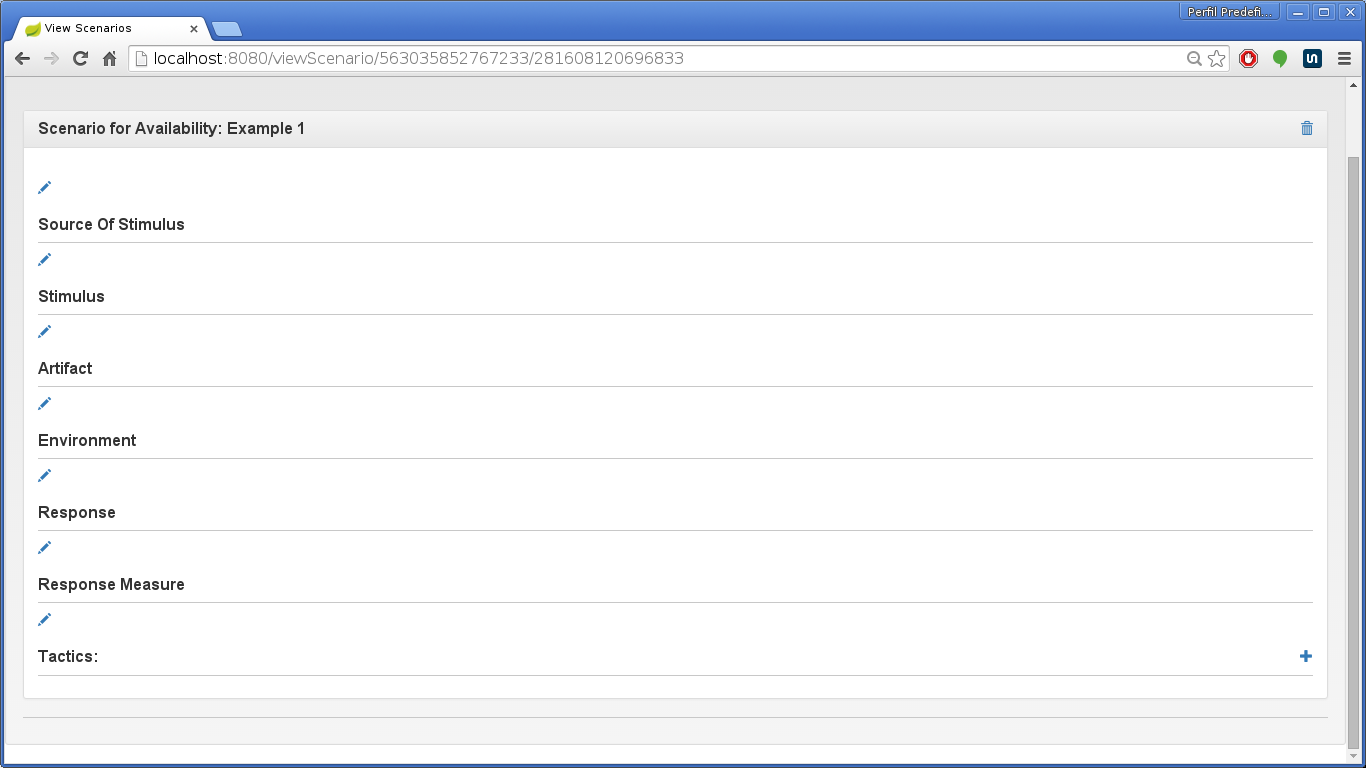
\includegraphics[width=15cm]{images/scenarioTemplate}
\centering
\caption{Template for a Scenario}
\label{figure:scenarioTemplate}
\end{figure}

The Views and their elements are also another case of main concepts. It makes sense to aggregate all the system elements and their relationships from a view in a separate template, representing the part of the system being described in that view. However, since a single element can be present in more than one view, it also makes sense to have a specific template for the elements, so their individual properties can be seen.

Figure \ref{figure:moduleTemplate} shows the template created for the Module, which is a specific system element from the Module Viewtype. Besides the element details, their relationships with other elements (other Modules, in this specific example) are present in the template.

Figure \ref{figure:viewTemplate} shows the template created for views from the Module Viewtype. Although the template allows inserting a description for the view, its most important feature is the inclusion of other templates in it. As mentioned, a view aggregates a set of system elements and the relationships between them. As there is already a template for the element, the view will include a set of element templates - a template per element, with its respective information.

\begin{figure}
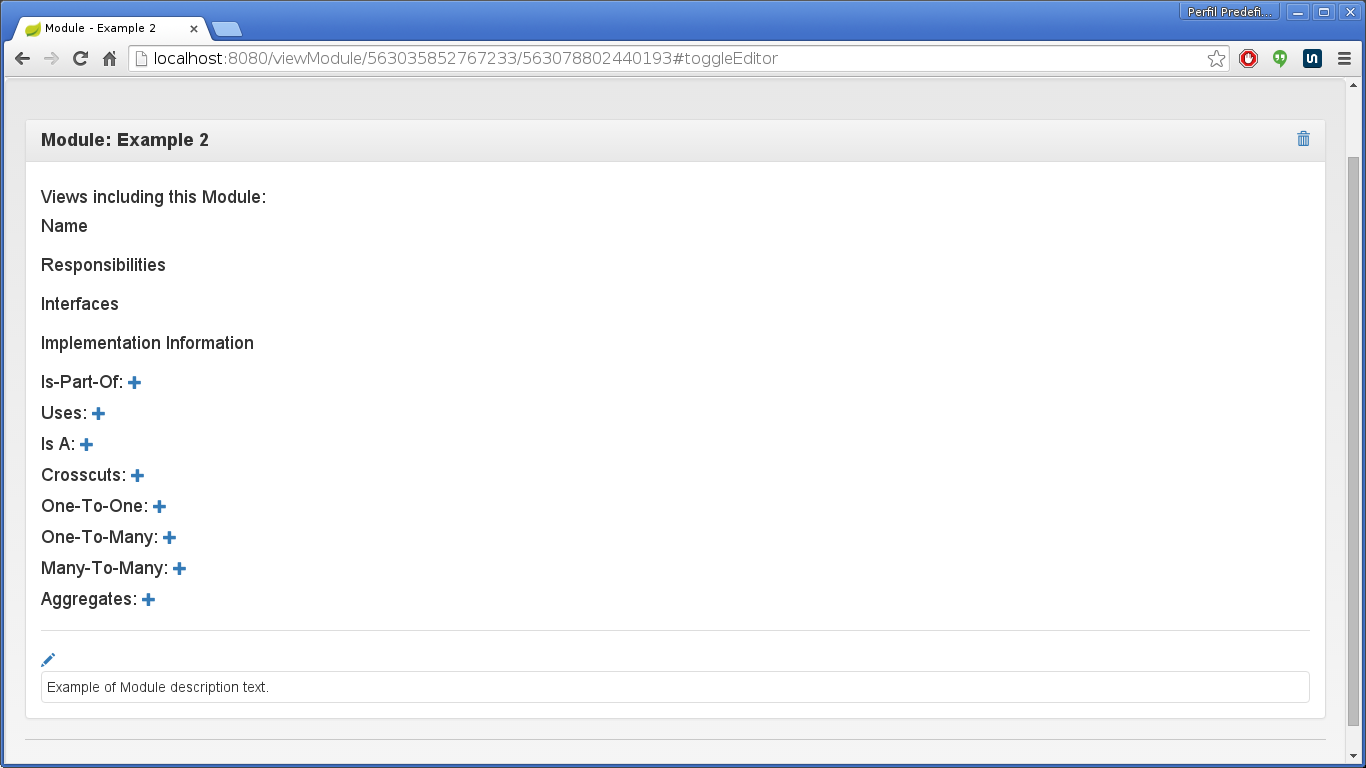
\includegraphics[width=15cm]{images/moduleTemplate}
\centering
\caption{Template for a Module}
\label{figure:moduleTemplate}
\end{figure}

\begin{figure}
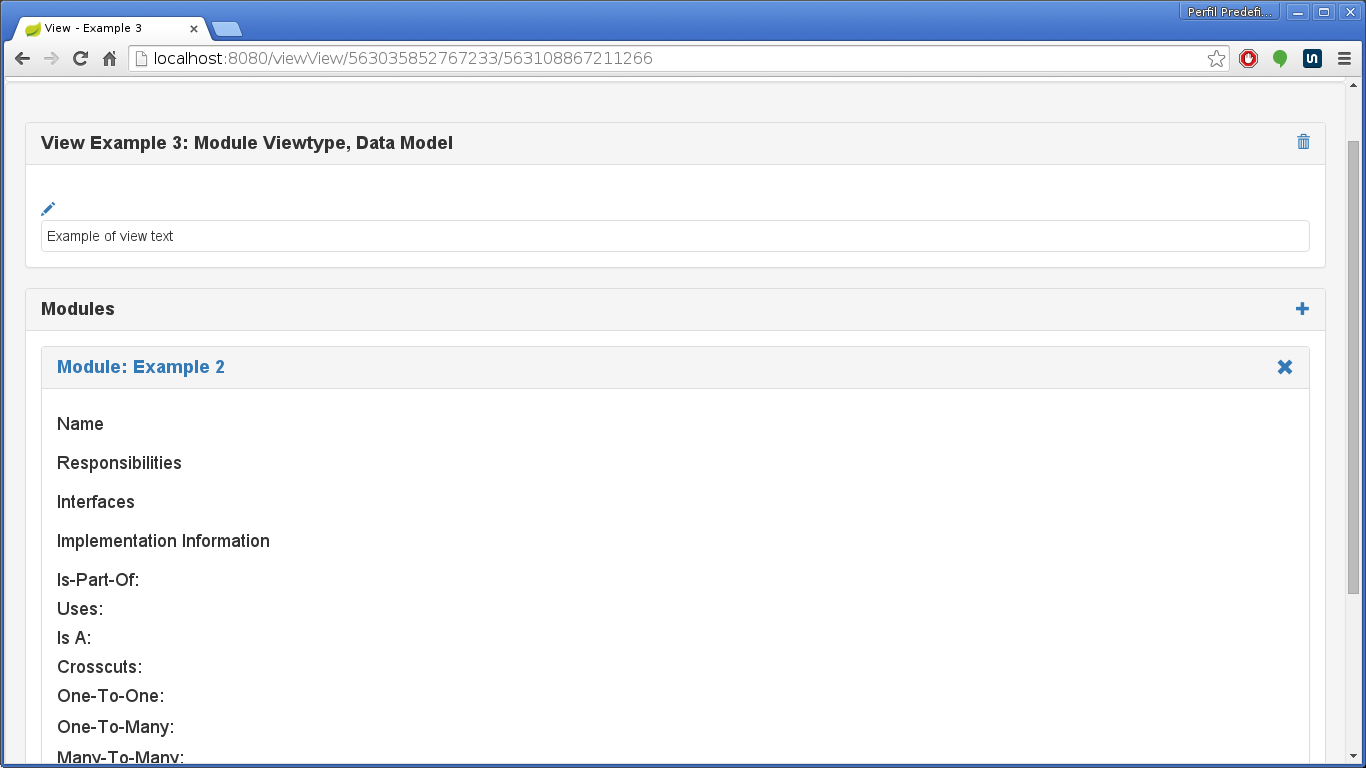
\includegraphics[width=15cm]{images/viewTemplate}
\centering
\caption{Template for a View}
\label{figure:viewTemplate}
\end{figure}


